% ==============================================================================



%% the first is for standalone compiling,
%%   the second looks for the master document

%\documentclass[classnotes]{fillsntsx}
\documentclass[../../../Master/AppliedStochastics.tex]{subfiles}


% ==============================================================================


%% without the master file this macro does nothing
%\course{Applied Stochastic Processes}


\author{Chandler}  % your name
\date{October 5}    % the date of the lecture


%% any custom macros should go here, but please be conservative
\usepackage{graphics} %for including images
\usepackage{float, subcaption} %for putting images where I want them, and not captioning them
\usepackage{kbordermatrix} %for labeling the matrix at the end of the notes 

\includeonly{../../../../macros}



% ==============================================================================
%
\begin{document}
%
% ==============================================================================


\makelecture % this is effectively \maketitle, the lecture follows


\section{An Application}
Sediment decomposition: 
Let $S_{k}$ = (amount of sediment deposited in year $k$) for $0\leq K \leq N=10^4$ 
and we model: 
$$\begin{aligned}
	S_{k+1} = \mu + (1-a) \cdot [S_{k}-\mu] + \eta_{k+1}
\end{aligned}$$
we could also write this as: 
$$\begin{aligned}
[S_{k+1}\vert S_{k} \sim N\big((1-a) \cdot [S_{k}-\mu], \sigma^2\big)]
\end{aligned}$$
Here $\eta_{k+1} \sim i.i.d N(0, \sigma^{2})$ where $\sigma^{2} = 10^{-4}$, and $a=10^{-3}$
So, $S_{k}$ with $\mu=0$ would look something like this: 
\begin{figure}[H]
	\centering
	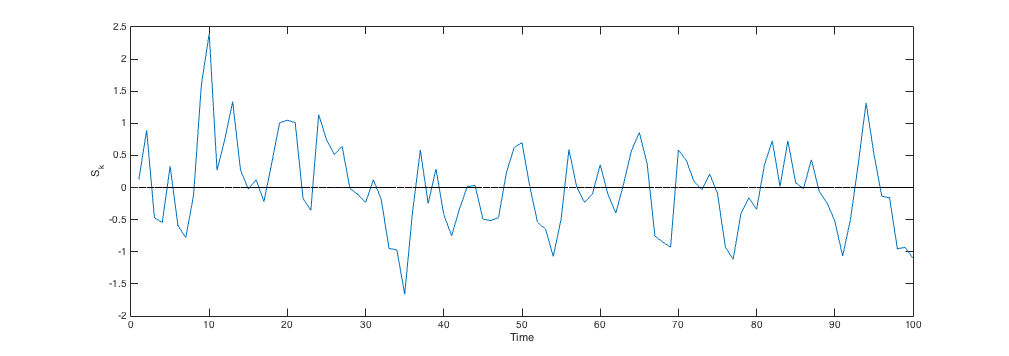
\includegraphics[width=0.7\linewidth]{process}
	\caption*{}
	\label{fig:process}
\end{figure}
As shown this is a process that stays distributed about a mean. 

Suppose we have noisy observations of $S_{t}$ for a few years 
Let $Y_{i}$ be our measurements 
$$\begin{aligned}
	Y_{i} = S_{k_{i}} + \varepsilon_{i}  
\end{aligned}$$
For $1 \leq i \leq N$ and $\varepsilon_{i} \sim i.i.d N(0, \sigma_{\varepsilon}^2)$ 
Our Goal: Estimate the total amount of sediment deposited 
$$\begin{aligned}
	S_{\mathrm{total}} = \sum_{k=1}^{N} S_{k}   
\end{aligned}$$
Let $D_{k} = S_{k}-\mu$ we can rewrite this as: 
$$\begin{aligned}
	D_{k} = \eta_{k} + (1-a)D_{k-1} =  \eta_{k} + (1-a)\eta_{k-1} + (1-a)^2 D_{k-2} = \sum_{j\geq0}(1-a)^j \eta_{k-j}
\end{aligned}$$
Thus, we know: 
$$\begin{aligned}
	D_{k}\sim N\bigg(0, \sigma^2 \cdot \sum_{j\geq0}(1-a)^2j\bigg) = N\bigg(0, \sigma^2 \dfrac{1}{(2-a)a}\bigg)
\end{aligned}$$
And since $\sigma^2 = 10^{-4}$ and $a=10^{-3}$ we can simplify this further, $D_{k} \sim N(0, \sim0.05)$. 
Let's say that $(W_{t})_{t\in\mathbb{R}}$ is a Brownian motion 
and $\eta_{k}= W_\frac{{k+1}}{N} - W_\frac{{k}}{N} \sim N\big(0, \frac{1}{N}=\sigma^2\big)$
Then, 
$$\begin{aligned}
	D_{k}= \sum_{j\geq0} (1-a)^j \Big(W_\frac{{k-j+1}}{N} - W_\frac{{k-j}}{N} \Big) \approx \sum_{j\geq0} e^{-aj} \Big(W_\frac{{k-j+1}}{N} - W_\frac{{k-j}}{N} \Big) = \int_{-\infty}^{t} e^{-aN(t-s)}dW_{s}
\end{aligned}$$
Where, $t=\frac{k}{N}$ and $0\leq t \leq 1$ 
Further simplifying we get, 
$$\begin{aligned}
D_{k}= \int_{-\infty}^{t} e^{-aN(t-s)}dW_{s} \sim N(0, \int_{-\infty}^{t}(e^{-aN(t-s)})^2 ds = \frac{1}{2aN}) \approx \frac{\sigma^2}{2a} + \mathcal{O}(a^2\sigma^2)
\end{aligned}$$
Let $U_{t} = \int_{-\infty}^{t} e^{-aN(t-s)} dW_{s}$ 
Also, $S_{\mathrm{total}}\simeq N\mu + \sum_{k=1}^{N} U_{\frac{k}{N}} \sim N\cdot(\mu + \int_{0}^{1}U_{t}dt)$

New question: Let $T=\int_{0}^{1} U_{t}dt$ 
and $X_{i} = U_{t_{i}} + \varepsilon_{i}$ where $\varepsilon_{i}\sim i.i.d N(0,\sigma_{\varepsilon}^2)$ 
What is the conditional distribution of $(T\vert X=X_{1},\dotso, X_{N}=X_{N})$ ? 

Now, we are trying to estimate the total integral, or the purple area below. 
\begin{figure}[H]
	\centering
	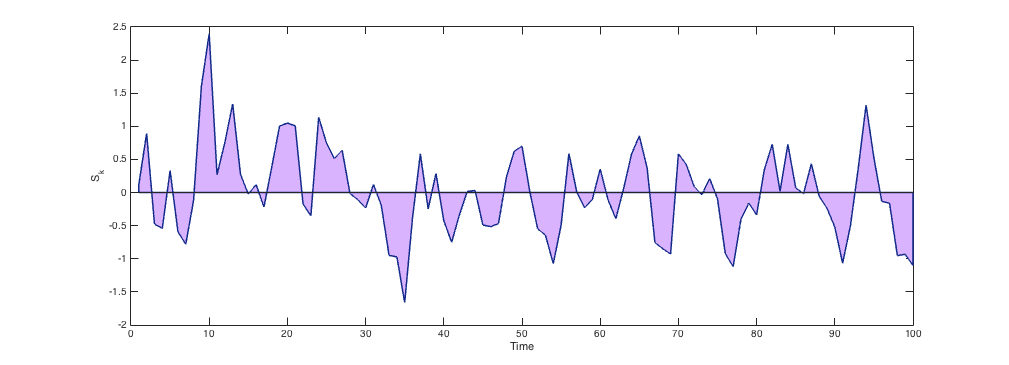
\includegraphics[width=0.7\linewidth]{area2}
	\caption*{}
	\label{fig:area2}
\end{figure}
The points on the blue curve are values of $U_{t}$, 
and the purple area is: $\int_{0}^{1} U_{t}dt = T$ 
To do this we need everything inside to be jointly Gaussian. 
i.e. we need to use the same white noise. 

Using the lemma from last lecture, 
we only need their covariance to calculate this area.
Recall the lemma,
if $(X,Y)$ is $N\Bigg(0, \begin{bmatrix} \Sigma_{XX}' & \Sigma_{XY} \\ \Sigma_{YX} & \Sigma_{YY}\end{bmatrix}\Bigg)$
then, $(X\vert Y=y) \sim N(\Sigma_{XY}\Sigma_{YY}^{-1}y, \Sigma_{XX}-\Sigma_{XY}\Sigma_{YY}^{-1}\Sigma_{XY}^{\intercal})$
To apply this we first need to expand $T$ 
$$\begin{aligned}
T = \int_{0}^{1} U_{t}dt = \int_{0}^{1}\int_{-\infty}^{t} e^{-aN(t-s)} dW_{s}dt 
=\int_{-\infty}^{1}\int_{\max(s,0)}^{t} e^{-aN(t-s)} dtdW_{s}\\
=\int_{-\infty}^{1} \frac{1}{aN}e^{aN\min(0,s)}\big(1-e^{-aN}\big)dW_{s}\coloneqq \int_{-\infty}^{1}\varphi(s)dW_{s}
\end{aligned}$$ 
Now, we know the following: 
$$\begin{aligned}
\var[T] = \int_{-\infty}^{1} \varphi^{2}(s) ds 
\end{aligned}$$ 

$$\begin{aligned}
\var[X_{i}] = \var[U_{t_{i}}] + \sigma_{\varepsilon} = \frac{1}{2aN} + \sigma_{\varepsilon}^2 
\end{aligned}$$ 

$$\begin{aligned}
\cov[X_{i}, X_{j}] = \int_{-\infty}^{t_{i}}e^{-aN(t_{i}-s)}\cdot e^{-aN(t_{j}-s)} ds = \frac{1}{2aN}[e^{-aN(t_{j}-t_{i})}]
\end{aligned}$$

for $i\neq j$ and $t_{i}<t_{j}$ 
Thus, 
$$\begin{aligned}
\cov[X_{i}, T] = \int_{-\infty}^{t} e^{-aN(t_{i}-s)}\varphi(s) ds 
\end{aligned}$$
where, 
$$\begin{aligned}
\Sigma = 
\begin{bmatrix}
  &  &  &  &  \\
 \vert\vert\varphi^2\vert\vert & 0 & \dotso & \dotso & 0 \\
 0 & \frac{1}{2aN}+\varepsilon^2 & 0 & \dotso & 0 \\
 0 & 0 & \ddots & \hfill & 0\\
 \vdots & \vdots & \vdots & \ddots & \vdots \\
 0 & 0 & 0 & 0 & \frac{1}{2aN}+\varepsilon^2
\end{bmatrix}
\end{aligned}$$
Where the columns are associated with $T$, $X_{1}$, $X_{2}$, and so forth. 
And the rows are similarly associated with $T$, $X_{1}$, $X_{2}$, and so forth. 
(This means the diagonal elements are the variances of $T$, $X_{1}$, $X_{2}$, $\dotso$, $X_N$).
% ==============================================================================
%
\end{document}
%
% ==============================================================================
